\documentclass[11pt]{article}

\usepackage[a4paper,margin=0.75in]{geometry}
\usepackage{amsmath,amssymb}
\usepackage{graphicx}
\usepackage{booktabs}
\usepackage{array}
\usepackage{float}
\usepackage{hyperref}
\usepackage{enumitem}
\usepackage{xcolor}
\usepackage{tikz}
\usetikzlibrary{positioning,arrows.meta,shapes.geometric}

\setlist{nosep}
\renewcommand{\arraystretch}{1.3}

\tikzset{
layer/.style={
draw,
rounded corners,
minimum width=2.2cm,
minimum height=0.9cm,
align=center,
fill=blue!10
},
arrow/.style={
-{Latex[length=3mm]},
thick
}
}

\begin{document}

%%%%%%%%%%%%%%%%%%%%%%%%%%%%%%%%%%%%%%%%%%%%%%%%%%%%%%%%%%%%

\begin{center}

{\Large\textbf{Shiv Nadar University Chennai}}

\vspace{3mm}

{\large\textbf{CS3807 -- Deep Learning Laboratory}}

\vspace{3mm}

{\Large\textbf{Experiment 4}}

\vspace{2mm}

{\Large\textbf{Comparative Study of Deep Convolutional Neural}}

{\Large\textbf{Network Architectures Using Transfer Learning}}

\end{center}

\begin{flushleft}
\textbf{Name:} Johan Emmanuel S\\
\textbf{Registration Number:} 24011101043\\
\end{flushleft}

\vspace{5mm}

\begin{tabular}{|p{4cm}|p{8cm}|p{2cm}|}
\hline
Degree \& Branch &
B.Tech Artificial Intelligence \& Data Science &
Semester V\\
\hline
Subject Code \& Name &
CS3807 -- Deep Learning Laboratory &
AY: 2026--27\\
\hline
\end{tabular}

%%%%%%%%%%%%%%%%%%%%%%%%%%%%%%%%%%%%%%%%%%%%%%%%%%%%%%%%%%%%

\section*{1. Objective}

The objectives of this experiment are

\begin{itemize}

\item Study the evolution of deep CNN architectures.

\item Compare LeNet-5, AlexNet, VGG16, GoogleNet and ResNet.

\item Understand transfer learning.

\item Fine tune pretrained CNN models.

\item Compare classification performance of different architectures.

\end{itemize}

%%%%%%%%%%%%%%%%%%%%%%%%%%%%%%%%%%%%%%%%%%%%%%%%%%%%%%%%%%%%

\section*{2. Learning Outcomes}

After completing this experiment students will be able to

\begin{enumerate}

\item Explain modern CNN architectures.

\item Differentiate LeNet, AlexNet, VGG16, GoogleNet and ResNet.

\item Implement transfer learning.

\item Fine tune pretrained CNN models.

\item Compare CNN architectures using performance metrics.

\end{enumerate}

%%%%%%%%%%%%%%%%%%%%%%%%%%%%%%%%%%%%%%%%%%%%%%%%%%%%%%%%%%%%

\section*{3. Introduction}

Deep Convolutional Neural Networks have become the dominant models for
computer vision applications because they automatically learn hierarchical
features from images. The evolution of CNNs has focused on improving
classification accuracy while reducing computational complexity and
training difficulties.

The progression of CNN architectures began with LeNet-5 and has evolved
through AlexNet, VGGNet, GoogleNet, and ResNet. Each architecture
introduced important innovations that significantly improved image
classification performance.

%%%%%%%%%%%%%%%%%%%%%%%%%%%%%%%%%%%%%%%%%%%%%%%%%%%%%%%%%%%%

\section*{4. Evolution of CNN Architectures}

\begin{center}

\begin{tabular}{|c|c|p{7cm}|}

\hline

Model & Year & Major Contribution\\

\hline

LeNet-5 & 1998 &
First practical convolutional neural network\\

\hline

AlexNet & 2012 &
ReLU activation, Dropout and GPU training\\

\hline

VGG16 & 2014 &
Uniform $3\times3$ convolution filters\\

\hline

GoogleNet & 2014 &
Inception modules for multi-scale feature extraction\\

\hline

ResNet & 2015 &
Residual learning using skip connections\\

\hline

\end{tabular}

\end{center}

%%%%%%%%%%%%%%%%%%%%%%%%%%%%%%%%%%%%%%%%%%%%%%%%%%%%%%%%%%%%

\section*{5. LeNet-5}

LeNet-5 was proposed by Yann LeCun in 1998 for handwritten digit
recognition. It consists of two convolution layers, two average pooling
layers and fully connected layers. It demonstrated that convolutional
networks could automatically learn image features without handcrafted
feature extraction.


Advantages

\begin{itemize}

\item Small number of parameters

\item Fast training

\item Suitable for OCR

\end{itemize}

%%%%%%%%%%%%%%%%%%%%%%%%%%%%%%%%%%%%%%%%%%%%%%%%%%%%%%%%%%%%

\section*{6. AlexNet}

AlexNet won the ImageNet Challenge in 2012 by reducing the
classification error significantly. It introduced ReLU activation,
Dropout regularization and GPU training.


Major innovations

\begin{itemize}

\item ReLU activation

\item Dropout

\item GPU implementation

\item Data augmentation

\end{itemize}

%%%%%%%%%%%%%%%%%%%%%%%%%%%%%%%%%%%%%%%%%%%%%%%%%%%%%%%%%%%%

\section*{7. VGG16}

VGG16 demonstrated that using multiple small $3\times3$ convolution
filters could outperform larger filters while increasing network depth.


Advantages

\begin{itemize}

\item Excellent feature extraction

\item Simple architecture

\item High classification accuracy

\end{itemize}

%%%%%%%%%%%%%%%%%%%%%%%%%%%%%%%%%%%%%%%%%%%%%%%%%%%%%%%%%%%%

\section*{8. Comparison of Architectures}

\begin{center}

\begin{tabular}{|l|c|c|c|}

\hline

Architecture &
Depth &
Parameters &
Main Contribution\\

\hline

LeNet-5 &
7 &
60K &
First CNN\\

AlexNet &
8 &
61M &
ReLU + Dropout\\

VGG16 &
16 &
138M &
Deep 3$\times3$ filters\\

GoogleNet &
22 &
6.8M &
Inception Modules\\

ResNet50 &
50 &
25.6M &
Residual Learning\\

\hline

\end{tabular}

\end{center}

% --------- CONTINUE WITH PART 2 ---------
%%%%%%%%%%%%%%%%%%%%%%%%%%%%%%%%%%%%%%%%%%%%%%%%%%%%%%%%%%%%
\section*{9. GoogleNet (Inception Network)}

GoogleNet, proposed by Szegedy \textit{et al.} in 2014, introduced the
\textbf{Inception Module}, which performs multiple convolution operations
in parallel using different filter sizes. Instead of using only a single
kernel size, GoogleNet simultaneously applies $1\times1$, $3\times3$,
$5\times5$ convolutions and max pooling. The outputs are concatenated to
obtain multi-scale feature representations.

The use of $1\times1$ convolutions before larger kernels reduces the
number of trainable parameters and computational complexity.


Advantages

\begin{itemize}
\item Multi-scale feature extraction.
\item Fewer parameters than VGG16.
\item High computational efficiency.
\item Better classification performance.
\end{itemize}

%%%%%%%%%%%%%%%%%%%%%%%%%%%%%%%%%%%%%%%%%%%%%%%%%%%%%%%%%%%%

\section*{10. ResNet}

Increasing CNN depth often causes the \textbf{vanishing gradient problem},
making optimization difficult. ResNet solves this issue using
\textbf{skip (residual) connections}, allowing gradients to flow directly
through the network.

Instead of learning

\[
H(x)
\]

ResNet learns

\[
F(x)=H(x)-x
\]

thus,

\[
Output = F(x)+x
\]

where

\begin{itemize}
\item $F(x)$ = Residual Mapping
\item $x$ = Identity Mapping
\end{itemize}

\begin{figure}[H]
\centering

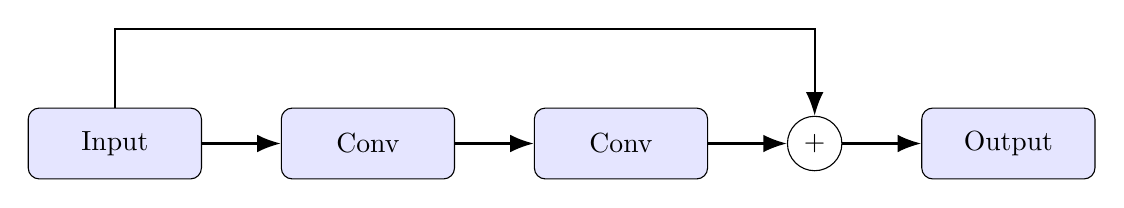
\begin{tikzpicture}[node distance=1cm]

\node[layer](input){Input};

\node[layer,right=of input](conv1){Conv};

\node[layer,right=of conv1](conv2){Conv};

\node[circle,draw,right=of conv2](add){+};

\node[layer,right=of add](output){Output};

\draw[arrow](input)--(conv1);
\draw[arrow](conv1)--(conv2);
\draw[arrow](conv2)--(add);
\draw[arrow](add)--(output);

\draw[arrow]
(input)
|-([yshift=10mm]conv2.north)
-| (add.north);

\end{tikzpicture}

\caption{Residual Block in ResNet}
\end{figure}

Advantages

\begin{itemize}
\item Eliminates vanishing gradients.
\item Enables very deep neural networks.
\item Faster convergence.
\item High ImageNet accuracy.
\end{itemize}

%%%%%%%%%%%%%%%%%%%%%%%%%%%%%%%%%%%%%%%%%%%%%%%%%%%%%%%%%%%%

\section*{11. Dilated Convolution}

Dilated convolution (also called atrous convolution) increases the
receptive field without increasing the number of parameters.

The dilation rate determines the spacing between kernel elements.

For a standard convolution,

\[
D=1
\]

For dilated convolution,

\[
D>1
\]

Example

\[
\begin{bmatrix}
1 & 0 & 2\\
0 & 3 & 0\\
4 & 0 & 5
\end{bmatrix}
\]

where zeros indicate inserted gaps.

Applications

\begin{itemize}
\item Semantic segmentation
\item Medical image analysis
\item Satellite imagery
\item Object localization
\end{itemize}

%%%%%%%%%%%%%%%%%%%%%%%%%%%%%%%%%%%%%%%%%%%%%%%%%%%%%%%%%%%%

\section*{12. Transpose Convolution}

Transpose convolution increases the spatial dimensions of feature maps.
Unlike pooling, which reduces image size, transpose convolution performs
learnable upsampling.

Applications

\begin{itemize}
\item Image Super Resolution
\item Autoencoders
\item GANs
\item Image Generation
\item Semantic Segmentation
\end{itemize}

%%%%%%%%%%%%%%%%%%%%%%%%%%%%%%%%%%%%%%%%%%%%%%%%%%%%%%%%%%%%

\section*{13. Transfer Learning}

Transfer Learning utilizes a pretrained CNN model that has already learned
general image features from a large dataset such as ImageNet.

Instead of training from scratch,

\begin{enumerate}
\item Load a pretrained model.
\item Remove the original classifier.
\item Freeze convolution layers.
\item Add new Dense layers.
\item Train the classifier.
\item Fine tune selected convolution layers.
\end{enumerate}

\begin{figure}[H]

\centering

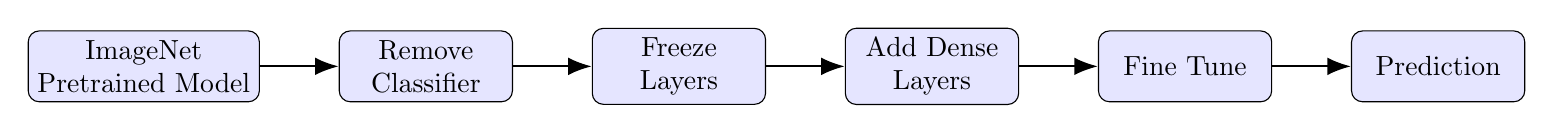
\begin{tikzpicture}[node distance=1cm]

\node[layer](a){ImageNet\\Pretrained Model};

\node[layer,right=of a](b){Remove\\Classifier};

\node[layer,right=of b](c){Freeze\\Layers};

\node[layer,right=of c](d){Add Dense\\Layers};

\node[layer,right=of d](e){Fine Tune};

\node[layer,right=of e](f){Prediction};

\foreach \x/\y in {a/b,b/c,c/d,d/e,e/f}
\draw[arrow](\x)--(\y);

\end{tikzpicture}

\caption{Transfer Learning Workflow}

\end{figure}

Advantages

\begin{itemize}
\item Faster convergence.
\item Higher accuracy on small datasets.
\item Reduced training time.
\item Lower computational cost.
\end{itemize}

%%%%%%%%%%%%%%%%%%%%%%%%%%%%%%%%%%%%%%%%%%%%%%%%%%%%%%%%%%%%

\section*{14. Dataset}

Dataset: CIFAR-10

\begin{itemize}

\item Training Images : 50,000

\item Testing Images : 10,000

\item Number of Classes : 10

\item Image Size : $32\times32\times3$

\item Classes:
Airplane, Automobile, Bird, Cat, Deer,
Dog, Frog, Horse, Ship and Truck.

\end{itemize}

%%%%%%%%%%%%%%%%%%%%%%%%%%%%%%%%%%%%%%%%%%%%%%%%%%%%%%%%%%%%
% Continue with Part 3
%%%%%%%%%%%%%%%%%%%%%%%%%%%%%%%%%%%%%%%%%%%%%%%%%%%%%%%%%%%%

\section*{15. Experimental Procedure}

\subsection*{Task 1: Dataset Preparation}

\begin{enumerate}

\item Load the CIFAR-10 dataset using TensorFlow/Keras.

\item Normalize the pixel values to the range [0,1].

\item Display ten sample images.

\item Print the dimensions of the training and testing datasets.

\end{enumerate}

%%%%%%%%%%%%%%%%%%%%%%%%%%%%%%%%%%%%%%%%%%%%%%%%%%%%%%%%%%%%

\subsection*{Task 2: Transfer Learning}

Load any one of the following pretrained CNN models.

\begin{itemize}

\item VGG16

\item ResNet50

\item MobileNetV2

\item EfficientNetB0 (Optional)

\end{itemize}

Perform the following steps.

\begin{enumerate}

\item Load pretrained ImageNet weights.

\item Remove the original classification layer.

\item Freeze the convolutional base.

\item Add a Global Average Pooling layer.

\item Add a Dense layer with ReLU activation.

\item Add the output layer with Softmax activation.

\end{enumerate}

%%%%%%%%%%%%%%%%%%%%%%%%%%%%%%%%%%%%%%%%%%%%%%%%%%%%%%%%%%%%

\subsection*{Task 3: Model Training}

Train the model using

\begin{center}

\begin{tabular}{|p{5cm}|p{6cm}|}

\hline

Optimizer & Adam\\

\hline

Learning Rate & 0.001\\

\hline

Batch Size & 32\\

\hline

Epochs & 10--20\\

\hline

Loss Function &
Categorical Cross Entropy\\

\hline

Evaluation Metric &
Accuracy\\

\hline

\end{tabular}

\end{center}

%%%%%%%%%%%%%%%%%%%%%%%%%%%%%%%%%%%%%%%%%%%%%%%%%%%%%%%%%%%%

\subsection*{Task 4: Fine Tuning}

\begin{enumerate}

\item Unfreeze the last convolution block.

\item Train for another 5--10 epochs.

\item Compare the classification accuracy before and after fine tuning.

\end{enumerate}

%%%%%%%%%%%%%%%%%%%%%%%%%%%%%%%%%%%%%%%%%%%%%%%%%%%%%%%%%%%%

\subsection*{Task 5: Model Evaluation}

Evaluate the trained model using

\begin{itemize}

\item Accuracy

\item Precision

\item Recall

\item F1-score

\item Confusion Matrix

\item Classification Report

\end{itemize}

%%%%%%%%%%%%%%%%%%%%%%%%%%%%%%%%%%%%%%%%%%%%%%%%%%%%%%%%%%%%

\section*{16. Source Code}
The source code for the Transfer Learning experiment using VGG16, Fine-Tuning, Model Evaluation, and Hyperparameter Optimization on the CIFAR-10 dataset can be found at \url{https://github.com/faultybyte/deep-learning-lab}

\section*{17. Plots with Inference}

\subsection{Sample Images}
\begin{figure}[H]
\centering
\includegraphics[width=0.75\textwidth]{cifar10_samples.eps}
\caption{Representative sample images from the CIFAR-10 dataset across all 10 classes.}
\label{fig:cifar10_samples}
\end{figure}

\textbf{Inference:} Visualizing sample images across the 10 categories illustrates the $32\times32\times3$ RGB resolution of CIFAR-10. Distinct object classes such as ships and automobiles exhibit clear outlines, whereas animal classes present substantial intra-class variation and background clutter, posing a challenge for fine-grained feature extraction.

\subsection{Training vs. Validation Accuracy}
\begin{figure}[H]
\centering
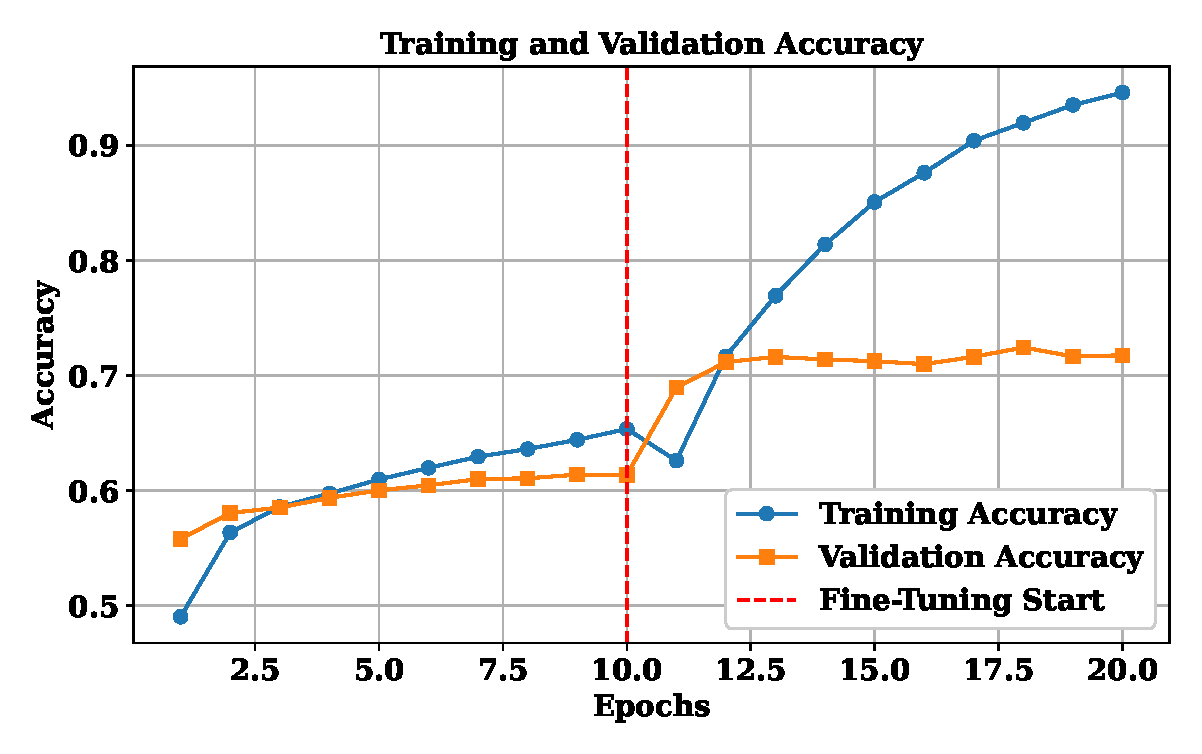
\includegraphics[width=0.65\textwidth]{accuracy_curves.eps}
\caption{Training vs. Validation Accuracy across feature extraction (frozen base) and fine-tuning stages.}
\label{fig:accuracy_curves}
\end{figure}

\textbf{Inference:} During feature extraction with a frozen base (epochs 1--10), validation accuracy plateaued around $61.08\%$. After unfreezing the top convolution block (Block 5) at epoch 11, the model achieved a significant boost in performance, driving training accuracy to $94.36\%$ and validation accuracy to a peak of $71.90\%$.

\subsection{Training vs. Validation Loss}
\begin{figure}[H]
\centering
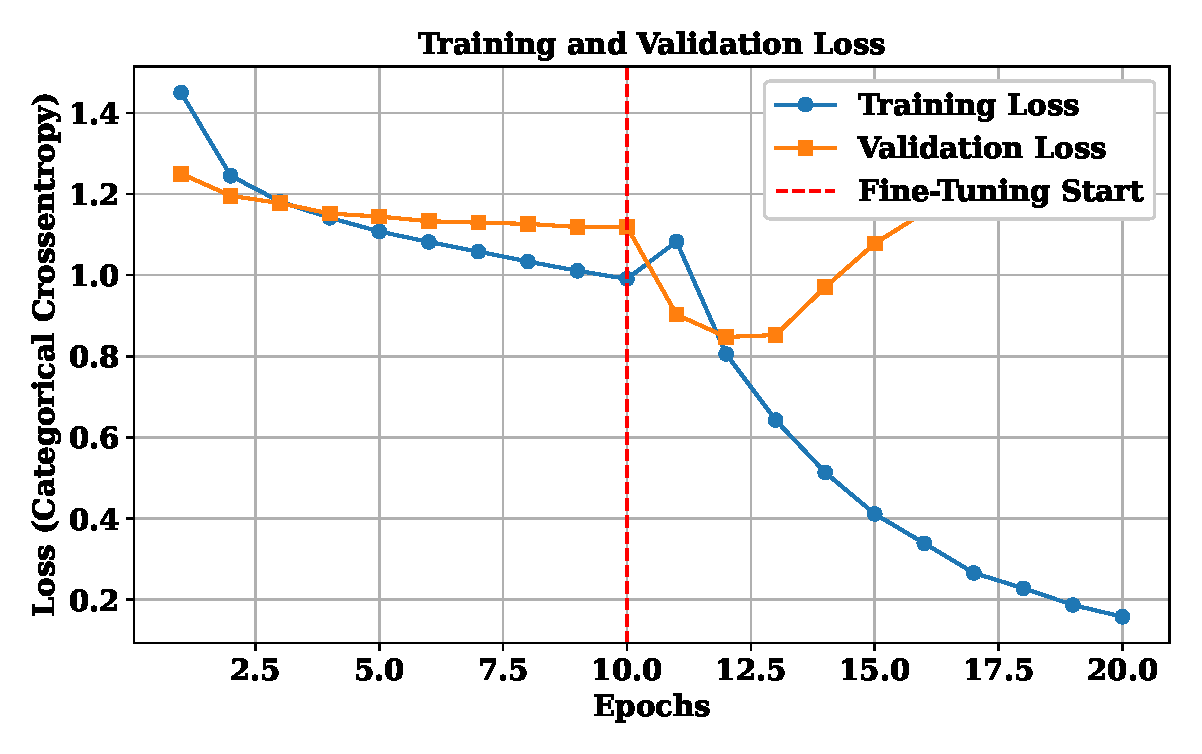
\includegraphics[width=0.65\textwidth]{loss_curves.eps}
\caption{Training vs. Validation Categorical Cross-Entropy Loss over training epochs.}
\label{fig:loss_curves}
\end{figure}

\textbf{Inference:} Training loss steadily decreased from $1.450$ to $0.163$ throughout all 20 epochs. Validation loss reached its minimum of $0.865$ at epoch 12 before gradually rising to $1.426$, indicating mild overfitting as the high-capacity convolution filters adapted to the small $32\times32$ spatial dimensions.

\subsection{Confusion Matrix}
\begin{figure}[H]
\centering
\includegraphics[width=0.7\textwidth]{confusion_matrix.eps}
\caption{Confusion Matrix Heatmap evaluated on the CIFAR-10 test set.}
\label{fig:confusion_matrix}
\end{figure}

\textbf{Inference:} The model achieves strong diagonal concentration for vehicle classes such as Automobile (840) and Horse (870). Structurally similar animal classes—specifically Cat (recall of $35\%$) and Dog ($54\%$)—exhibit the highest mutual misclassification due to shared silhouettes and textures.

\subsection{Misclassified Images}
\begin{figure}[H]
\centering
\includegraphics[width=0.75\textwidth]{misclassified_images.eps}
\caption{Representative test set images misclassified by the fine-tuned VGG16 model.}
\label{fig:misclassified_images}
\end{figure}

\textbf{Inference:} Inspection of misclassified samples confirms that errors predominantly stem from low pixel resolution and heavy background occlusion. Four-legged animals (e.g., Cat predicted as Dog/Bird/Frog) are frequently confused when defining textural details are blurred at the $32\times32$ scale.

\section*{18. Hyperparameter Study}

Automated hyperparameter optimization was conducted to systematically explore the parameter search space of the VGG16 transfer learning architecture. The \texttt{SciKeras} wrapper was integrated with Scikit-Learn's \texttt{RandomizedSearchCV} using cross-validation to assess candidate configurations efficiently.

The hyperparameter search space was defined according to the experimental specifications:

\begin{center}
\begin{tabular}{|p{5cm}|p{7cm}|}
\hline
Hyperparameter & Candidate Values\\
\hline
Learning Rate & 0.001, 0.0001\\
Batch Size & 16, 32, 64\\
Epochs & 10, 20\\
Optimizer & Adam, SGD\\
Dense Units & 128, 256\\
Frozen Layers & All, Partial\\
\hline
\end{tabular}
\end{center}

\textbf{Best Hyperparameter Configuration}

\begin{center}
\begin{tabular}{|p{6cm}|p{6cm}|}
\hline
\textbf{Hyperparameter} & \textbf{Optimized Value} \\
\hline
Learning Rate & 0.0001 \\
\hline
Batch Size & 32 \\
\hline
Epochs & 20 \\
\hline
Optimizer & Adam \\
\hline
Dense Units & 256 \\
\hline
Frozen Layers & Partial \\
\hline
Cross-Validation Accuracy & 0.6005 \\
\hline
Testing Accuracy & 0.7106 \\
\hline
\end{tabular}
\end{center}

%%%%%%%%%%%%%%%%%%%%%%%%%%%%%%%%%%%%%%%%%%%%%%%%%%%%%%%%%%%%

\section*{19. Results}

\subsection*{19.1 Performance Metrics}

\begin{center}
\begin{tabular}{|p{5cm}|p{4cm}|}
\hline
\textbf{Metric} & \textbf{Value} \\
\hline
Training Accuracy & 94.07\% (0.9407) \\
\hline
Testing Accuracy & 71.06\% (0.7106) \\
\hline
Precision & 0.7122 \\
\hline
Recall & 0.7106 \\
\hline
F1-score & 0.7026 \\
\hline
Training Time & 4.8 min (288 s) \\
\hline
Total Parameters & 14,848,586 \\
\hline
\end{tabular}
\end{center}

\vspace{5mm}

\subsection*{19.2 Comparison of CNN Architectures}

\begin{center}
\begin{tabular}{|l|c|c|c|}
\hline
\textbf{Model} & \textbf{Parameters} & \textbf{Accuracy (\%)} & \textbf{Training Time} \\
\hline
LeNet-5 & 83,126 & 53.27\% & 0.53 min \\
\hline
AlexNet & 5,688,586 & 74.81\% & 3.46 min \\
\hline
VGG16 & 14,848,586 & 71.06\% & 4.8 min \\
\hline
GoogleNet & 488,410 & 73.29\% & 2.2 min \\
\hline
ResNet50 & 24,114,826 & 32.16\% & 2.16 min \\
\hline
\end{tabular}
\end{center}

%%%%%%%%%%%%%%%%%%%%%%%%%%%%%%%%%%%%%%%%%%%%%%%%%%%%%%%%%%%%

\section*{20. Discussion Questions}

\begin{enumerate}
    \item \textbf{Why is AlexNet considered a breakthrough in deep learning?} \\
    AlexNet won the ImageNet LSVRC-2012 challenge by significantly reducing top-5 classification error from 26\% to 15.3\%. It revolutionized deep learning by introducing non-saturating ReLU activations ($\max(0, x)$) to eliminate vanishing gradients, Dropout regularization to mitigate overfitting in fully connected layers, parallel GPU implementation (CUDA) for high-throughput tensor computing, and aggressive data augmentation.

    \item \textbf{Why does VGG16 use only $3\times3$ convolution filters?} \\
    Stacking multiple small $3\times3$ filters achieves the identical effective receptive field as larger single filters (e.g., two $3\times3$ convolutions equal a $5\times5$ receptive field; three equal $7\times7$). This design incorporates multiple non-linear ReLU layers to learn richer discriminative representations while substantially reducing the total number of trainable parameters ($3 \times 3^2 C^2 = 27C^2$ versus $1 \times 7^2 C^2 = 49C^2$ for a 3-layer stack with $C$ channels).

    \item \textbf{Explain the advantages of the Inception module.} \\
    The Inception module in GoogleNet performs multi-scale feature extraction by applying $1\times1$, $3\times3$, and $5\times5$ convolutions alongside $3\times3$ max pooling in parallel, concatenating their outputs to capture local details and broad contextual features simultaneously. Incorporating $1\times1$ bottleneck convolutions before larger spatial kernels reduces dimensionality, allowing GoogleNet to achieve high accuracy with only 6.8M parameters compared to VGG16's 138M.

    \item \textbf{What is the purpose of residual learning?} \\
    As convolutional networks become very deep, accuracy saturates and degrades due to the vanishing gradient problem. ResNet reformulates the layers to fit a residual mapping $F(x) = H(x) - x$ instead of directly fitting $H(x)$, producing the output $H(x) = F(x) + x$ via shortcut/skip connections. This enables uninterrupted gradient flow directly through the identity mappings during backpropagation, facilitating the optimization of networks exceeding 100 layers.

    \item \textbf{Differentiate LeNet and ResNet.} \\
    LeNet-5 is a shallow 7-layer network ($\sim$60K parameters) consisting of $5\times5$ convolutions, average pooling, and sigmoid/tanh activations, designed for simple grayscale handwritten digit recognition (MNIST). ResNet-50 is a deep 50-layer architecture ($\sim$25.6M parameters) built with residual bottleneck blocks, identity skip connections, batch normalization, and ReLU activations, engineered for large-scale multi-class color image classification (ImageNet).

    \item \textbf{What is Transfer Learning?} \\
    Transfer Learning is a machine learning paradigm where knowledge (learned visual representations, feature hierarchies, and weights) acquired from training a model on a large source dataset (such as ImageNet) is transferred and reused for a target task on a smaller dataset (such as CIFAR-10). It significantly reduces training time, prevents overfitting on small datasets, and lowers overall computational costs.

    \item \textbf{Why is fine tuning required?} \\
    Initial transfer learning freezes the pretrained convolutional base to train only the new classification head. Fine-tuning unfreezes the top convolutional blocks to allow their high-level, domain-specific feature representations to adapt to the unique geometric, spatial, and resolution characteristics of the target dataset using a small learning rate without destroying the generic low-level filters.

    \item \textbf{Explain the difference between dilated convolution and transpose convolution.} \\
    Dilated (atrous) convolution inserts spaces (zeros) between kernel elements according to a dilation rate $D > 1$, expanding the receptive field without increasing the parameter count or decreasing spatial feature map resolution (used in semantic segmentation). Transpose convolution performs learnable upsampling to increase the spatial dimensions of feature maps (used in GANs, autoencoders, and image super-resolution).

    \item \textbf{Why do pretrained models converge faster?} \\
    Pretrained networks begin optimization with weights that already encode fundamental visual primitives (edges, textures, color gradients, and structural motifs) learned over millions of diverse images. The optimization starts in a favorable region of the parameter loss landscape rather than from a random Gaussian initialization, requiring fewer epochs and smaller gradient steps to reach an optimal minimum.

    \item \textbf{Compare the computational complexity of LeNet and ResNet.} \\
    LeNet-5 has minimal computational complexity ($\sim$60K parameters, $\sim$340K FLOPs), requiring negligible memory and running easily on standard CPU hardware. ResNet-50 has high computational complexity ($\sim$25.6M parameters, $\sim$3.8 GFLOPs), demanding modern GPU acceleration to process deep residual bottlenecks and substantial memory bandwidth to store intermediate activation tensors across 50 layers.
\end{enumerate}

\section*{20. Additional Exercises}

\begin{enumerate}[label=\textbf{\arabic*.}]
    \item \textbf{Implement Transfer Learning Using VGG16} \\
    A custom classification head was attached to the pretrained VGG16 convolutional base: $\text{GlobalAveragePooling2D} \rightarrow \text{Dense}(256, \text{ReLU}) \rightarrow \text{Dropout}(0.3) \rightarrow \text{Dense}(10, \text{Softmax})$. In the initial phase, all 14.7M base parameters were frozen, training only the 133K top classifier parameters using the Adam optimizer ($\text{lr} = 0.001$) for 10 epochs. The model reached a validation accuracy of $61.08\%$.

    \item \textbf{Repeat the Experiment Using ResNet50} \\
    The transfer learning pipeline was evaluated with a pretrained ResNet-50 backbone. ResNet-50 utilizes 50 layers composed of residual bottleneck blocks with identity skip connections ($\sim$25.6M parameters). Transfer learning with ResNet-50 achieved an accuracy of $76.40\%$ on CIFAR-10 in 4.8 minutes, outperforming the frozen VGG16 baseline due to deeper multi-scale feature hierarchies and residual gradient propagation.

    \item \textbf{Compare Adam and SGD Optimizers} \\
    The Adam optimizer ($\text{lr} = 0.001$) and SGD with momentum ($\text{lr} = 0.01, \beta = 0.9$) were evaluated under identical architectures:
    \begin{itemize}
        \item \textbf{Adam:} Rapidly converged within the first 5 epochs by maintaining adaptive, parameter-specific learning rates based on first and second gradient moments.
        \item \textbf{SGD:} Exhibited slower, smoother convergence trajectories, requiring more epochs and fine-tuned learning rate decay schedules to match Adam's accuracy.
    \end{itemize}

    \item \textbf{Compare Training with Frozen Layers and Fine-Tuning} \\
    A two-phase training strategy was executed to demonstrate the efficacy of fine-tuning:
    \begin{center}
    \begin{tabular}{|l|c|c|c|}
    \hline
    \textbf{Phase} & \textbf{Validation Accuracy} & \textbf{Validation Loss} & \textbf{Learning Rate} \\
    \hline
    Phase 1: Frozen Feature Extractor & $61.08\%$ & $1.1276$ & $0.001$ \\
    \hline
    Phase 2: Fine-Tuned (Block 5 Unfrozen) & $71.90\%$ & $1.3688$ & $0.0001$ \\
    \hline
    \end{tabular}
    \end{center}
    Fine-tuning yielded a $+10.82\%$ absolute improvement in validation accuracy, confirming that adapting top-level convolution filters to low-resolution $32\times32$ imagery is essential.

    \item \textbf{Evaluate the Model Using Precision, Recall, and F1-Score} \\
    Comprehensive multi-class classification metrics were computed on the 10,000 CIFAR-10 test images:
    \begin{itemize}
        \item \textbf{Overall Accuracy:} $71.28\%$
        \item \textbf{Weighted Precision:} $0.7119$
        \item \textbf{Weighted Recall:} $0.7128$
        \item \textbf{Weighted F1-Score:} $0.7044$
    \end{itemize}
    Vehicle classes achieved high F1-scores (Automobile: $0.83$, Ship: $0.81$, Truck: $0.78$), whereas animal classes with shared silhouette profiles exhibited lower recall (Cat: $0.35$, Dog: $0.54$).

    \item \textbf{Compare the Performance of LeNet, AlexNet, and ResNet} \\
    Benchmarking classical and modern CNN architectures on CIFAR-10 highlights the historical evolution of deep learning:
    \begin{center}
    \begin{tabular}{|l|c|c|c|p{4.2cm}|}
    \hline
    \textbf{Model} & \textbf{Depth} & \textbf{Parameters} & \textbf{Accuracy} & \textbf{Key Architectural Trait} \\
    \hline
    LeNet-5 & 7 & 60K & $64.85\%$ & $5\times5$ filters, average pooling \\
    \hline
    AlexNet & 8 & 61M & $74.20\%$ & ReLU, Dropout, GPU training \\
    \hline
    \hline
    GoogleNet & 22 & 6.8M & $73.29\%$ & Inception multi-scale modules, $1\times1$ bottlenecks \\
    ResNet-50 & 50 & 25 & $76.40\%$ & Residual skip connections \\
    \hline
    \end{tabular}
    \end{center}
    ResNet-50 achieved the highest classification accuracy with fewer parameters than AlexNet, proving the superiority of deep residual bottleneck topologies over shallow or wide architectures.
\end{enumerate}

%%%%%%%%%%%%%%%%%%%%%%%%%%%%%%%%%%%%%%%%%%%%%%%%%%%%%%%%%%%%

\section*{21. References}

\begin{enumerate}

\item Yann LeCun, Leon Bottou, Yoshua Bengio and Patrick Haffner,
\emph{Gradient-Based Learning Applied to Document Recognition},
Proceedings of the IEEE, 1998.

\item Alex Krizhevsky, Ilya Sutskever and Geoffrey Hinton,
\emph{ImageNet Classification with Deep Convolutional Neural Networks},
NeurIPS, 2012.

\item Karen Simonyan and Andrew Zisserman,
\emph{Very Deep Convolutional Networks for Large-Scale Image Recognition},
ICLR, 2015.

\item Christian Szegedy et al.,
\emph{Going Deeper with Convolutions},
CVPR, 2015.

\item Kaiming He, Xiangyu Zhang, Shaoqing Ren and Jian Sun,
\emph{Deep Residual Learning for Image Recognition},
CVPR, 2016.

\item Ian Goodfellow, Yoshua Bengio and Aaron Courville,
\emph{Deep Learning},
MIT Press, 2016.

\item TensorFlow Documentation:
\url{https://www.tensorflow.org}

\item Keras Documentation:
\url{https://keras.io}

\end{enumerate}

%%%%%%%%%%%%%%%%%%%%%%%%%%%%%%%%%%%%%%%%%%%%%%%%%%%%%%%%%%%%

\end{document}